\documentclass[letterpaper,10pt]{article}

%\setlength{\parindent}{0in}
%\usepackage{fullpage} 
\usepackage{amsmath}
\usepackage{amssymb}
\usepackage{enumerate}
\usepackage{graphicx}
\usepackage[table]{xcolor}
\usepackage{dcolumn}
\oddsidemargin 0.0in
\textwidth 6.5in
\newcolumntype{.}{D{.}{.}{-1}}
\newcommand*{\myalign}[2]{\multicolumn{1}{#1}{#2}}

%Project Assignment 1 (Module 5): (15 points – 12 points for the assignment 
%and 3 points for each individual role playing DB submission)
%Project Assignment 1 Requirements Analysis is a team event and is due 
%2/10/12.  Please see the Project Area on Sakai for more guidance.
%a. Identify and list primary stakeholders and determine stakeholder 
%requirements.
%b. Define the capability needs statement (what capability do we have now, what 
%capability do we need, what is the gap and how will be close the gap?) This is 
%similar to the effective need.
%c. Determine top level system requirements and KPPs. 
%d. As a result of your analysis rank the system requirements. Rank the highest 
%level system requirements based on operational stakeholder preferences.
%e. Prepare an OV-1: High-Level Operational Concept Graphic and a high-level 
%textual description of the operational concept.
%f. Prepare a SV-4 Systems Functionality Description Describe the functions 
%(activities) performed by systems and the system data flows among system 
%functions (activities).What insight does it provide about the system?
%g. Summarize and present the result of your analysis.
%Remember to complete your RPG Role Evaluation on the Discussion Board 
%also!
%Project Assignment 2 (Module 6): (15 points – 12 points for the assignment and 3 
%points for each individual role playing DB submission)

\title{Project 1 \\ \Large Team CLEAR \\ \normalsize (Convoy Level Explosive Ammunition Removal)}
\author{Christian Aall: Testing \& Evaluation \\ 
	Steve Mazza: Team Lead \\ 
	Michael Oexmann: Analyst \\ 
	Elizabeth Swisher: Lead Systems Engineer}
	
\date{February 10, 2012}

\begin{document}
\maketitle

Researching warfighter needs with regard to the area clearing of improvised explosive devices (IEDs), we arrive at an identification of stakeholders and stakeholder requirements, top-level system requirements, and key performance parameters (KPPs) for the METAL-V system.  Ranking the top-level system requirements allows us to help prioritize the systems engineering effort across the development of this project.  Development of a capability needs statement focuses us and drives our collective understanding of the warfighter need and outcomes necessary to judge success or failure at the platform level.  Lastly, we provide high-level contextual and system documentation.

\section{Stakeholders and Stakeholder Requirements}
\subsection{Stakeholders}
The following stakeholders were derived directly from the project documentation.
\begin{itemize}
	\item Systems Engineering Experts, Inc. (SEE, Inc.)
	\item Testers-R-Us (responsible for testing the prototype against requirements)
	\item Contracting Companies (competing in advanced development prototype competition)
	\item Warfighter (the end user)
	\item Taxpayer (financial support)
	\item Congress (budget approval)
	\item PEO-IED (where our IPT works)
	\item Lego, Inc. (manufactures a critical component used to create METAL-V)
\end{itemize}
The following suggests an additional list of stakeholders not specifically referenced but who, nonetheless, should be considered.
\begin{itemize}
	\item PEO C3T
	\item PM Mission Command
	\item Tank Automotive Research, Development and Engineering Center's (TARDEC)
	\item Project Manager Close Combat Systems (PM CCS)
	\item Product Manager Countermine and Explosive Ordnance Disposal (PdM CM\&EOD)
	\item Product Manager IED Defeat/Protect Force (IEDD/PF)
\end{itemize}

\subsection{Stakeholder Requirements}
The following sections define requirements by stakeholder and are presented in no particular order.

\begin{itemize}
	\item Systems Engineering Experts, Inc. (SEE, Inc)
	\begin{itemize}
		\item SEE licensed software tools shall be utilized to analyze the product.
	\end{itemize}
	\item Testers-R-Us
	\begin{itemize}
		\item System shall be tested against Limited Objective Exercise (LOE) objectives.
		\item System shall be tested demonstrating Technology Readiness Level (TRL).
	\end{itemize}
	\item Contracting Companies
	\begin{itemize}
		\item The assessment of alternatives shall be fairly weighted.
		\item The system performance rating system shall be clearly defined.
	\end{itemize}
	\item Warfighter
	\begin{itemize}
		\item The system shall meet acceptable reliability level.
		\item The system shall accurately detect explosives.
		\item The system shall meet acceptable available levels.
		\item The system shall meet acceptable ruggedized levels.
		\item The system shall demonstrate fast search coverage.
		\item The system shall be rapidly deployable by typical soldier/Marine.
		\item The system shall be easy to transport.
	\end{itemize}
	\item Taxpayer
	\begin{itemize}
		\item The system shall be researched and developed in the most cost effective process possible.
	\end{itemize}
	\item Congress
	\begin{itemize}
		\item The system shall meet agreed upon budgetary constraints.
		\item The system shall meet agreed upon schedule constraints.
	\end{itemize}
	\item PEO-IED
	\begin{itemize}
		\item METAL-V shall traverse designated area.
		\item System shall detect simulated IED.
		\item Simulated IED shall exhibit characteristics of IEDs found in theater.
	\end{itemize}
	\item Lego, Inc.:
	\begin{itemize}
		\item The system shall utilize the METAL-V to perform terrestrial locomotion
	\end{itemize}
\end{itemize}

\section{Capability Needs Statement}
While the warfighter presently relies on efficient and effective route clearing of improvised Explosive devices (IEDs), continued sustainment of operations in theater as well as protection of civilian lives hinges on the development of safe and effective area clearing capabilities.  The ability to detect IEDs within a defined area would result in a greater mission success rate by increasing the agility and flexibility of a mission over the current preferred alternative of IED detection, route clearance. 

Currently IED area clearance is still an immature technology but the recent advances in the Micro Expeditionary Transforming Air Land-Vehicle (METAL-V) offers a mature product that can be enhanced into an IED area clearance system by adapting its software to detect IEDs that display known characteristics. Development of this technology for application in theater relies on the Army's ability to leverage commercially available hardware, industry expertise, and existing government intellectual property (IP) and developed capabilities.  Utilizing a prototype system to prove the concept will ultimately shorted the time to fielding and increase Army acceptance.

\section{Ranked Top Level System Requirements and KPPs}
\subsection{Key Performance Parameters}
The table below summarized the key performance parameters for the METAL-V system.

\begin{center}
\begin{tabular}{lrr}
\hline
\myalign{c}{\textbf{Parameter}} & \myalign{c}{\textbf{Threshold}} & \myalign{c}{\textbf{Goal}} \\
\hline\hline
Mission Reliability (DRM) & 0.9 & 0.95 \\
Operational Availability & 0.8 & 0.9 \\
Life-cycle Cost per Unit & \$50,000 & \$25,000 \\
Vehicle Weight & 18 oz & 14 oz \\
Refueling Time & 60 sec. & 30 sec. \\
DRM Elapsed Time & 5 min. & 3 min. \\
Deployed-to-Ready Time & 10 min. & 5 min. \\
SMETAL-V Storage Container & 216 in$^{3}$ & 120 in$^{3}$ \\
Operational Team Size & 2 persons & 1 person \\
\hline
\end{tabular}
\end{center}

\subsection{Top-level System Requirements, Prioritized, of the METAL-V}
The following is a list of top-level system requirements that have been ranked (prioritized) based on the operational stakeholder's (end user's) preference.
\begin{enumerate}
	\item The system shall have a mission reliability of at least 0.90.
	\item The system shall have an operational availability of at least 0.80.
	\item The system shall never indicate a false negative.
	\item The system shall indicate a false positive less that 2\% of the time.
	\item The system shall successfully detect and distinguish 95\% of threats in a given area over a given time.
	\item The system shall successfully alert the IED-clearance operator of a threat 98\% of the time.
	\item The system shall require an average training period not to exceed 4 hours.
	\item The system's deployment-to-ready time shall not exceed 10 minutes.
	\item The system shall have an average usability score of at least 8 based on end-user input.
	\item The system shall require no more than 2 people to operate.
	\item The system shall not require any specialized parts or training for routine maintenance or repair.\footnote{We are treating the Lego Mindstorm Brick as a COTS product.}
	\item The system vehicle's weight shall not exceed 18 ounces.
	\item The system’s SMETAL-V storage container shall have a volume not to exceed 216 cubic inches.
	\item The system's DRM elapsed time shall not exceed 5 minutes.
	\item The system vehicle shall have a drop height of at least 1 inch.
	\item The refueling time of the system shall not exceed 60 seconds.
	\item The system's life-cycle cost shall not exceed \$50,000.
\end{enumerate}

\subsection{Explanation of Top-level System Requirement Prioritization}
The top-level system requirements have been prioritized based on operational stakeholder (end user) preference. The top priority of any user is typically safety. In this case, the operational stakeholder is most interested in the system's ability to correctly perform its mission to detect IEDs and therefore preventing fatal injury to the operator and other friendly personnel.

Following the system's correct operation, the operational stakeholder is probably most interested in \emph{how} the system will be operated. How much training is required? How long does the system take to deploy? How difficult is the system to use? These types of requirements are factors which directly impact the end user and play a role in user acceptance. Operational stakeholders must also consider the transport of the systems they use; therefore weight, volume, and drop height are areas of principal interest.

The system requirement having the lowest priority is life-cycle cost. As would be expected, the end user typically does not care how much a system costs as they are not directly responsible for payment. This requirement would have much higher priority, however, if viewed from a procurement office's point of view.

\section{Diagrams}
\begin{figure}[h!tbp]
	\begin{center}
		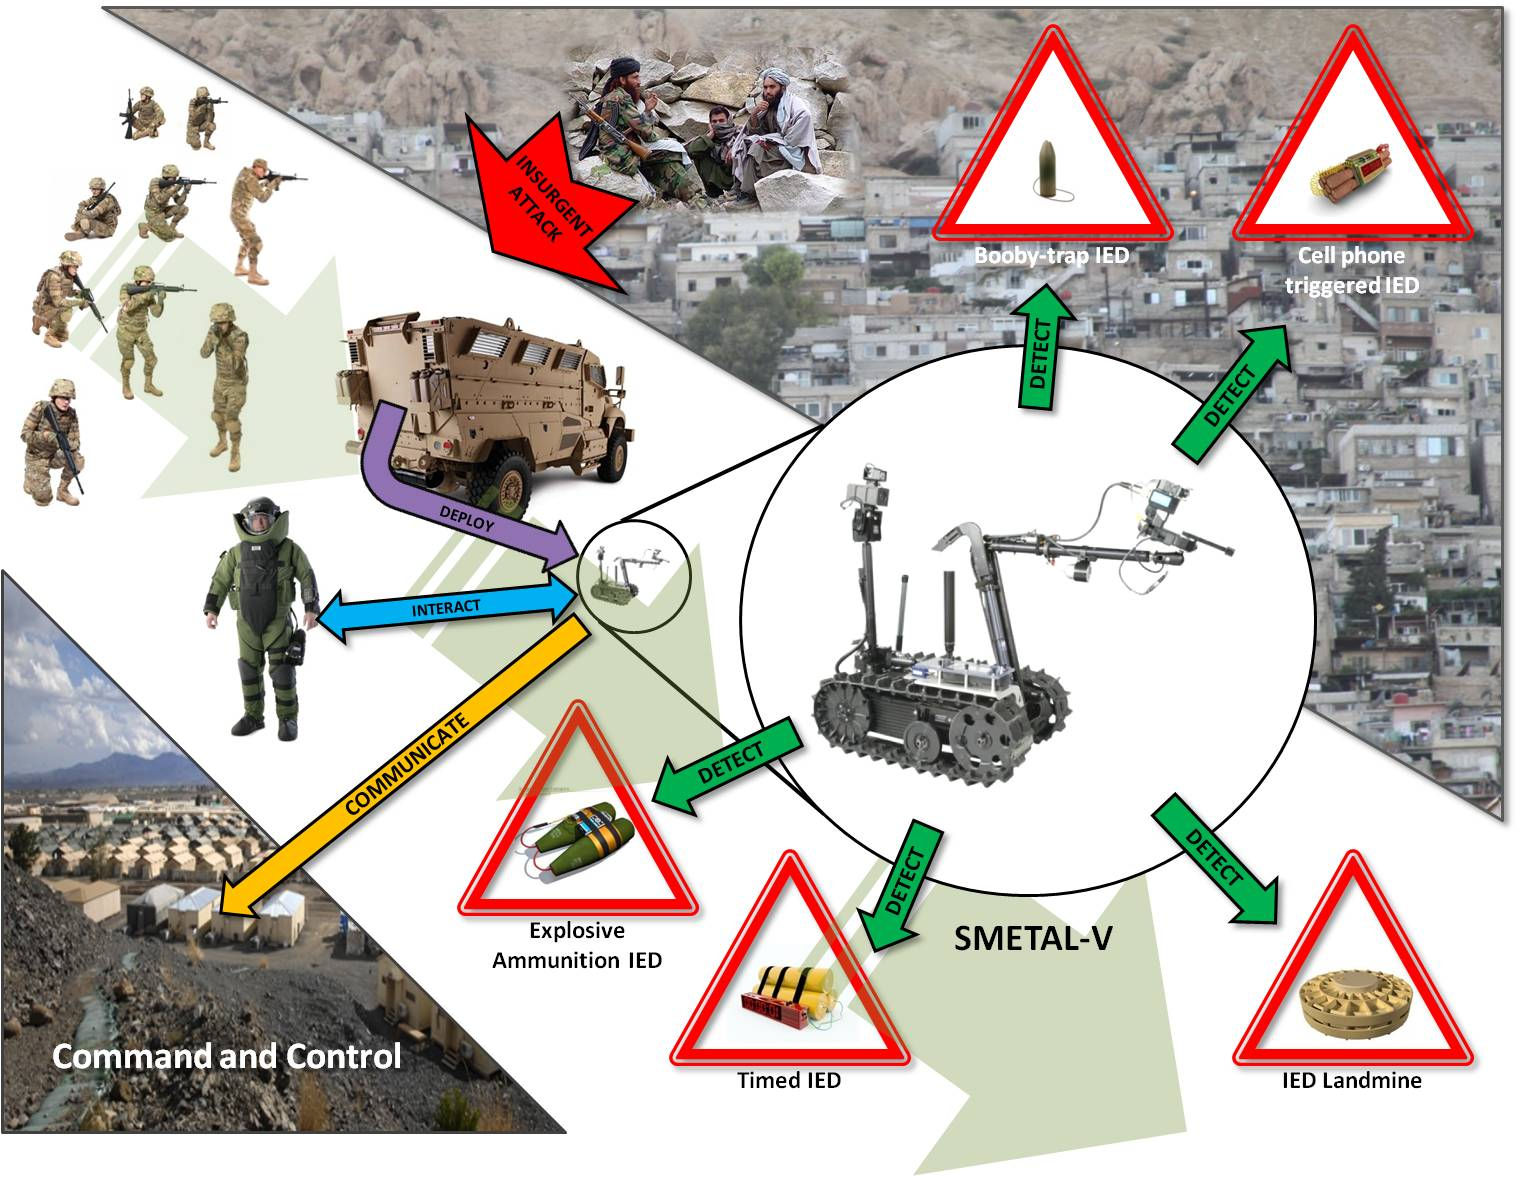
\includegraphics[scale=0.6]{ov1.jpg}
		\caption{OV-1}
	\end{center}
\end{figure}

%\section{SV-4}
The following figures lend insight into the system in several ways.  They provide us with an increased understanding of logical encapsulation of data and functionality that informs software best practices, modular design, distributed development, and component re-use.  Similarly, they help us to understand the physical encapsulation of functionality that informs modular design and manufacturing.

Since system timing and cohesiveness is critical to a well-functioning system and ultimately to a high mission success rate, it is important to note that the diagrams also inform our understanding of data flow needs including system timing requirements and lend an increased understanding of requirements for interoperability among component system parts.

\begin{figure}[h!tbp]
	\begin{center}
		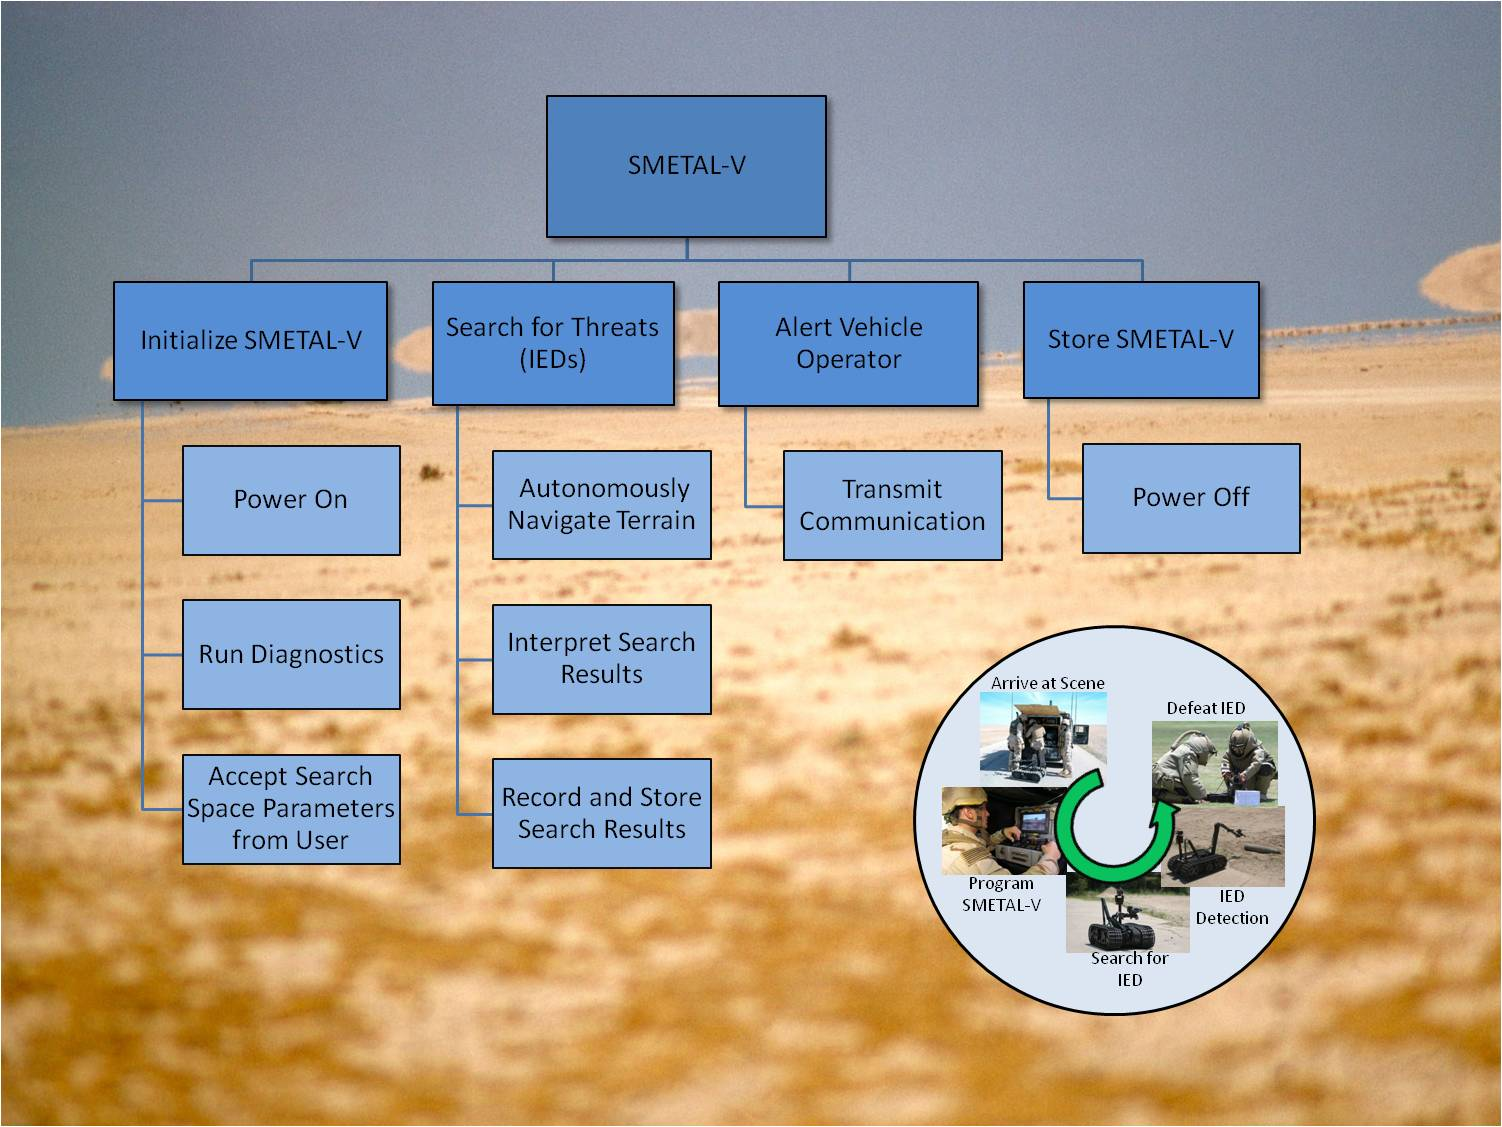
\includegraphics[scale=0.6]{sv4a.jpg}
		\caption{SV-4a}
	\end{center}
\end{figure}

\begin{figure}[h!tbp]
	\begin{center}
		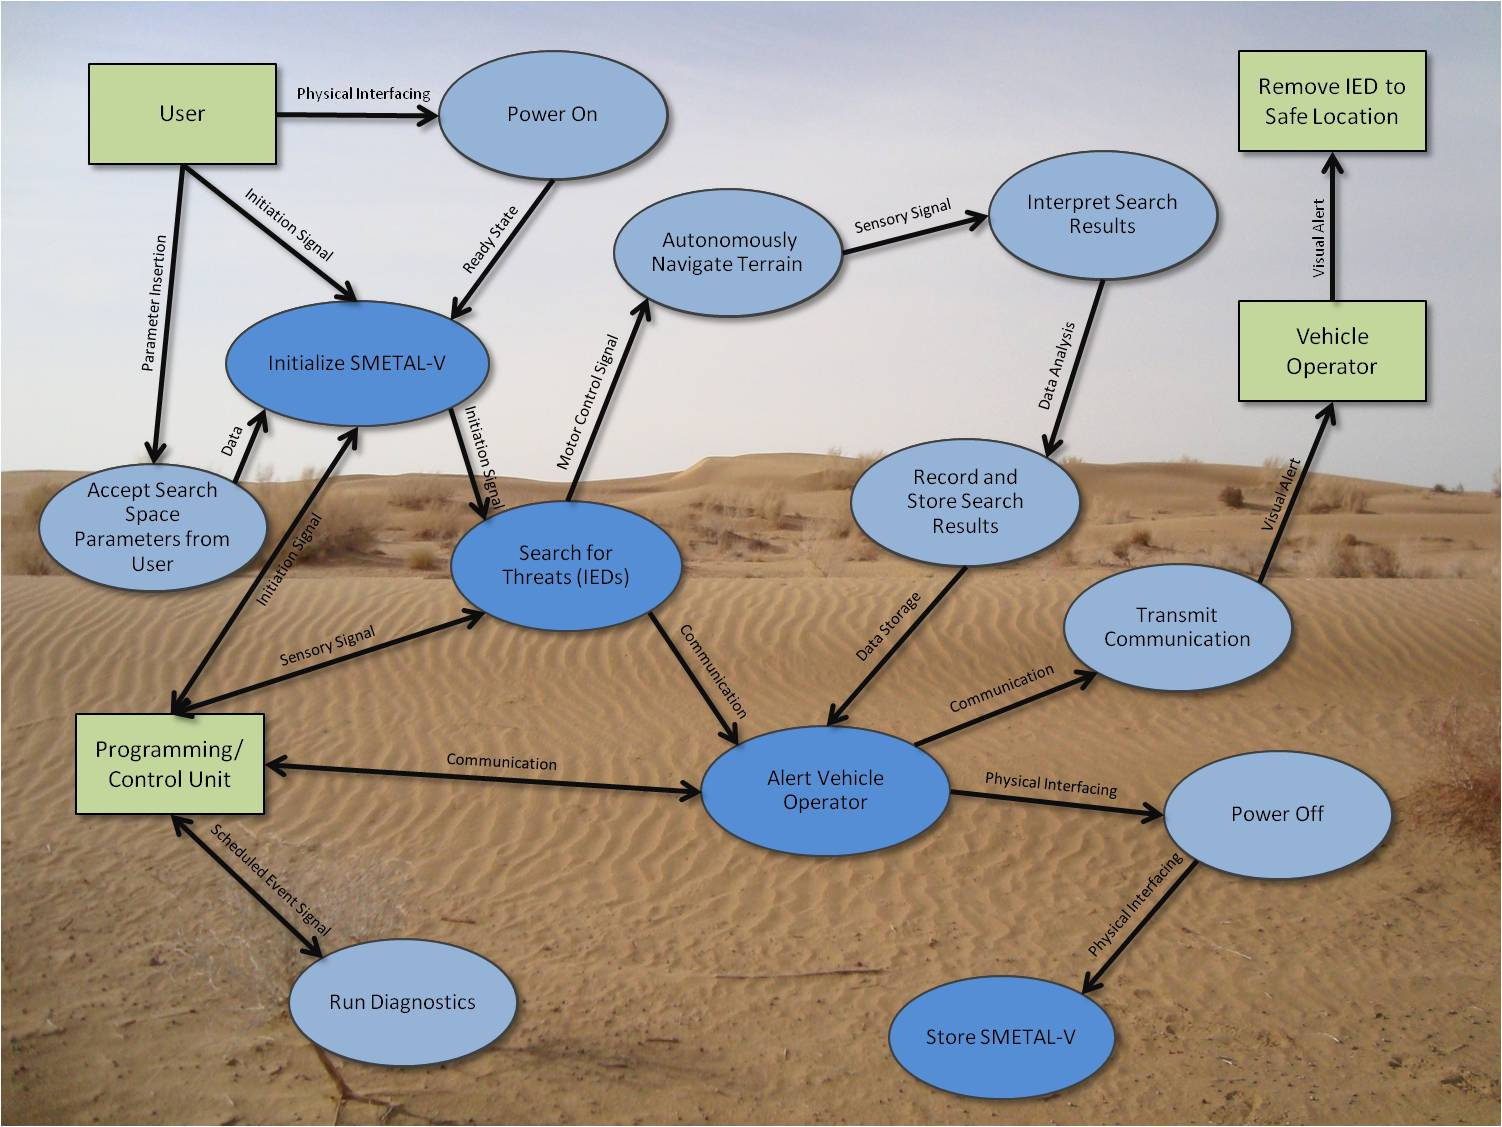
\includegraphics[scale=0.6]{sv4b.jpg}
		\caption{SV-4b}
	\end{center}
\end{figure}


\end{document}